\documentclass[12pt, twosided]{article}
\usepackage[letterpaper,bindingoffset=0in,%
            left=1in,right=1in,top=1in,bottom=1in,%
            footskip=.25in]{geometry}

\usepackage{mathtools}
\usepackage{graphicx}

\usepackage{setspace}
\setstretch{1.1}

\usepackage{amsmath}
\usepackage{amsfonts}
\usepackage{amsthm}
\usepackage{amssymb}
\usepackage{csquotes}
\usepackage{relsize}

\usepackage{tikz}
\usetikzlibrary{cd}
\usetikzlibrary{fit,shapes.geometric}
\tikzset{%  
    mdot/.style={draw, circle, fill=black},
    mset/.style={draw, ellipse, very thick},
}

\usepackage{hhline}
\usepackage{systeme}
\usepackage{mathrsfs}
\usepackage{hyperref}
\usepackage{mathtools}  
\usepackage{silence}
\usepackage{blkarray}
\usepackage{float}
\usepackage{framed}
\usepackage{array}
\usepackage{stmaryrd}
\usepackage{extarrows}
\usepackage{caption}
\captionsetup[figure]{labelfont={bf},name={Fig.},labelsep=period}

\theoremstyle{definition}
\newtheorem{df}{Definition}
\newtheorem{exa}{Example}
\newtheorem{ques}{Question}
\newtheorem{exr}{Exercise}
\newtheorem{prb}{Problem}
\newtheorem*{note}{Note}
\theoremstyle{plain}
\newtheorem{thm}{Theorem}
\newtheorem{prop}{Proposition}
\newtheorem{conj}{Conjecture}
\newtheorem{cor}{Corollary}
\newtheorem{lm}{Lemma}
\newtheorem*{fact}{Fact}
\newtheorem*{idea}{Idea}
\newtheorem*{clm}{Claim}
\newtheorem*{rmk}{Remark}
\usepackage[ruled]{algorithm2e}

\usepackage{ulem}
\makeatletter

\def\lf{\left\lfloor}   
\def\rf{\right\rfloor}
\def\lc{\left\lceil}   
\def\rc{\right\rceil}
\def\st{\text{ s.t. }}
\def\1{^{-1}}
\def\ind{\mathbf{1}}
\def\R{\mathbb{R}}
\def\Q{\mathbb{Q}}
\def\Z{\mathbb{Z}}
\def\C{\mathbb{C}}
\def\I{\mathbb{I}}
\def\N{\mathbb{N}}
\def\F{\mathbb{F}}
\def\A{\mathbb{A}}
\def\Li{\text{Li}}
\def\th{^\text{th}}
\def\sp{\text{Sp}}
\def\opn{\left\{}
\def\cls{\right\}}
\def\Aut{\text{Aut}}
\def\PG{\text{PG}}
\def\GL{\text{GL}}
\def\PGL{\text{PGL}}
\def\Cov{\text{Cov}}
\def\Pack{\text{Pack}}
\def\PgamL{\text{P}\Gamma\text{L}}
\def\gamL{\Gamma\text{L}}
\def\cl{\text{cl}}
\def\stbar{\ \middle\vert\ }
\def\partdone{\hphantom{1} \hfill \(\triangle\)}
\def\s0{_0}
\def\s1{_1}
\def\s2{_2}
\def\id{\mathrm{id}}
\def\topn{\text{ open}}
\def\Bd{\text{Bd }}
\def\nope{\(\longrightarrow\!\!\longleftarrow\)}
\def\stt{\(^{\text{st}}\ \)}
\def\tht{\(^{\text{th}}\ \)}
\def\ndt{\(^{\text{nd}}\ \)}
\renewcommand{\P}{\mathbb{P}}
\newcommand{\leg}[2]{\left( \frac{#1}{#2} \right)}

\renewcommand*\env@matrix[1][*\c@MaxMatrixCols c]{%
   \hskip -\arraycolsep
   \let\@ifnextchar\new@ifnextchar
   \array{#1}}
\makeatother

% These two lines suppress the warning generated 
% by amsmath for overwriting the choose command  
% because it's annoying. This probably has unint-
% ended ramifications somewhere else, but I'm too
% lazy to actually figure that out, so we'll cro-
% ss that bridge when we come to it lol.
\renewcommand{\choose}[2]{\left( {#1 \atop #2} \right)}
\WarningFilter{amsmath}{Foreign command} 

\renewcommand{\mod}[1]{\ (\mathrm{mod}\ #1)}
\renewcommand{\vec}[1]{\mathbf{#1}}

\let\oldprime\prime
\def\prime{^\oldprime}

\usepackage{float}
\restylefloat{figure}

\usepackage{cleveref}
\Crefname{thm}{Theorem}{Theorems}

% Comment commands for co-authors
\newcommand{\kmd}[1]{{\color{purple} #1}}

\newcolumntype{L}{>{$}l<{$}}
% Bib matter
\let\oldepsilon\epsilon
\def\epsilon{\varepsilon}

\let\oldphi\phi
\def\phi{\varphi}

%%% Local Variables:
%%% mode: plain-tex
%%% TeX-master: t
%%% End:

\graphicspath{{./img/}}

\begin{document}
\noindent \textbf{Math 171} \hfill \textbf{Professor Sebastian Bozlee} \\
\textbf{Scribed by: Kyle Dituro} \hfill \textbf{\today}\hrule
\vspace{.2in}

\begin{df}
  A subset \(I\) of \(\R\) is said to be convex if for any \(a, b \in I\) with \(a < b\), we have \([a,b] \subseteq I\).
\end{df}
\begin{exa}
  \(\emptyset\), \(\opn a \cls\), \((a,b)\), \((a, b]\), \([a,b), [a,b], [a, \infty), (a, \infty), (-\infty, a), (-\infty, a], (\infty, \infty)\).
\end{exa}

\begin{thm}
  A subspace \(I\) of \(\R\) is connected if and only if it is convex.
\end{thm}

\begin{proof}
  Suppose \(I\) is connected. Suppose for the sake of contradiction that \(I\) is not convex. Then \(\exists a,b \in I\), \(a < b\) such that \(\exists z\) with \(a < z < b\) and \(z \not\in I\).

  Consider \(U = (-\infty, z) \cap I\), \(V= (z, \infty) \cap I\).

  \(U, V\) are clearly disjoint and nonempty (since \(a \in U\) \(b \in V\) by construction), open, and have union \(I\).

  This is therefore a separation, and a contradiction. So \(I\) is convex.

  Now suppose \(I\) is convex. Suppose for contradiction that \(U, V\) is a separation of \(I\).

  Let \(a \in U, b\in V\). Now without loss of generality, assume that \(a < b\). Consider the interval \([a,b]\).

  Let

  a
  \begin{align*}
    U_0 = U \cap [a,b] \quad V_0 = V \cap [a, b].
  \end{align*}
  This is a separation. \(U_0, V_0\) are disjoint, open in \([a,b]\), nonempty since \(a \in U\), \(b \in V\), and their union is all of \([a,b]\).

  Let \(c = \sup U_0\)

  \begin{enumerate}
  \item [(Case 1):]\hspace{1em}

    \begin{center}
      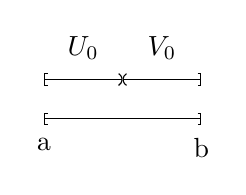
\begin{tikzpicture}[y=.5cm]
        \draw[Bracket-Bracket] (0, 0) -- (2,0) node[pos=0, label=below:a] {} node[pos=1, label=below:b] {};
        \draw[Bracket-Parenthesis] (0,1) -- (1,1) node[pos=.5, label=above:\(U_0\)] {};
        \draw[Parenthesis-Bracket] (1,1) -- (2,1) node[pos=.5, label=above:\(V_0\)] {};
      \end{tikzpicture}
    \end{center}
    Since \(U_0\) is open in \([a,b]\) and \(c < b\) and \(c \in U_0\), there is some \(d \in (a,b)\) such that \([c, d) \subseteq U_0\). But then \(\frac{c + d}{2} \in U_0\) and \(c < \frac{c + d}{2}\), so \(c\) is not an upper bound on \(U_0\), a contradiction.

    
  \item [(Case 2):] \((c \in V_0)\) Then \(c = b\) or \(a < c < b\).

    Since \(V_0\) is open in \([a,b]\) and \(a < c\), \(c \in V_0\), there is some \(e \in (a, b)\) such that \((e,c] \subseteq V_0\). Then \(e\) is an upper bound on \(U_0\), but this contradicts that \(c\) is the least upper bound on \(U_x\).
    
  \end{enumerate}

  Now \(c \not\in U_0\) and \(c \not\in V_0\), so \([a,b] \neq U_0 \cup V_0\), and thus \(I\) is connected.
\end{proof}

\begin{thm}[Intermediate Value Theorem]
  Let \(f: X \to \R\) be a continuous function where \(X\) is a connected topological space. Then if \(a, b\in X\) and \(y\) is between \(f(a)\) and \(f(b)\), then there exists \(c \in X\) such that \(f(c) = y\). 
\end{thm}

\begin{proof}
  Since \(X\) is connected and \(f\) is continuous, \(f(X)\) is connected. By the previous theorem, \(f(X)\) is convex, so \(y \in f(X)\). Then by the definition of the image, \(\exists c \in X\) such that \(f(c) = y\).
\end{proof}

Now we will give yet another characterization of continuity. One that is perhaps a bit stronger than our prior ones, but should aide our intuition.

\begin{df}
  Let \(X\) be a topological space, \(p, q \in X\). A \textbf{path} from \(p\) to \(q\) in \(X\) is a continuous function \(f:[a,b] \to X\) such that \(f(a) = p\), \(f(b) = q\).

  We say that \(X\) is \textbf{path connected} if for any \(p,q\in X\) there is a path in \(X\) from \(p\) to \(q\).
\end{df}


\begin{prop}
  If \(X\) is path connected, then \(X\) is connected.
\end{prop}

\begin{proof}
  Suppose for the sake of contradiction that \(U, V\) is a separation of \(X\). Let \(p \in U, q \in V\). Since \(X\) is path connected, there is a continuous function \(f:[a,b] \to X\). Then \(f(a) = p\) and \(q = f(b)\). Then \(f([a,b])\) is connected since \([a,b]\) is connected.

  Then \(f([a,b]) \subseteq U\) or \(f([a,b])\subseteq V\), but this is impossible since \(p\not\in V\), \(q \not\in U\).
\end{proof}

\begin{exa}
  The unit ball \(B\) in \(\R^n\) is connected, since it is path connected.

  If \(\vec{p},\vec{q} \in B\), then \(
  \begin{matrix}
    f:[0,1] \to B \\ t \mapsto (1-t)\vec{p} + t\vec{q}
  \end{matrix}\) will be a path from \(\vec{p}\) to \(\vec{q}\).
\end{exa}

\begin{exa}[Connected \(\not\Rightarrow\) Path connected]\hspace{1em}

  \begin{center}
    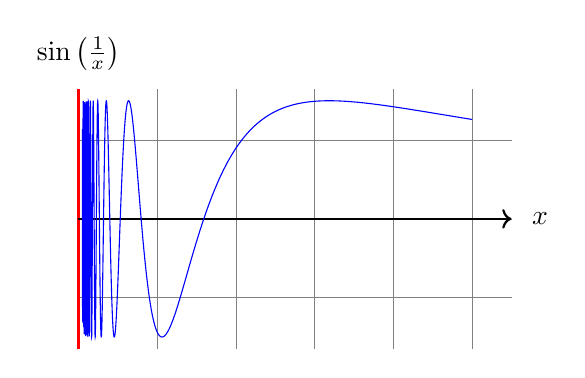
\begin{tikzpicture}[x=5cm, y=1.5cm]
      \draw[help lines] (0,-1.1) grid (1.1, 1.1);
      \draw[thick,red] (0,-1.1) -- (0,1.1);
      \node at (0,1.4) {\(\sin\left(\frac{1}{x}\right)\)};
      \draw[thick, ->] (0,0) -- (1.1,0) node[pos = 1, label=right:\(x\)] {};
      \draw[domain=.01:1, samples=5000, blue] plot (\x, {sin((1/\x)r)});
    \end{tikzpicture}
  \end{center}
  Let \(S = \opn (t, \sin\left(\frac{1}{t}\right) \stbar 0 < t \leq 1) \cls.\)

  This is connected, since it is the image of a connected space. Take the closure:

  \begin{align*}
    \overline{S} = \opn 0 \cls \times [-1, 1] \cup S
  \end{align*}
\end{exa}

\begin{fact}
  Closures of connected subspaces are also connected.
\end{fact}

Let \(\vec{p} = (0, 0)\), \(q = (1, \sin(1))\).

Suppose \(f: [0,1] \to \overline{S}\) is a path from \(\vec{p}\) to \(\vec{q}\).

notice \(0 \times [-1, 1]\) is a closed set, so its preimage under \(f\) is a closed set, with some max.

Reparameterizing, we may assume this max is \(0\).

By the intermediate value theorem, for each integer \(n > 0\), there is some \(t_n\) such that \(f(t_n) = \left(\frac{1}{2\pi n + \frac{\pi}{2}}. \sin\left(2\pi n + \frac{\pi}{2}\right)\right) = \left(\frac{1}{2\pi}, 1\right) \).

Then
\begin{align*}
  &\lim_{n \to \infty} f(t_n) = (0, 1) \neq f(0) = (0, 0) \\
  &\lim_{n \to \infty} t_n = 0
\end{align*}
\end{document}
%%% Local Variables:
%%% mode: latex
%%% TeX-master: t
%%% End:
